% Shared TikZ style for the architecture atlas. \input by the thesis preamble AND by each
% standalone compile-test wrapper, so diagrams render identically in both. Core libraries
% only (shadows.blend is unavailable in this TeX install).
\usetikzlibrary{positioning,arrows.meta,calc,fit,backgrounds,shapes.geometric,shapes.misc,decorations.pathreplacing}
\tikzset{
  % ---- node roles (colour = function; shared by every diagram) -------------------------
  blk/.style   ={draw,rounded corners=2.2pt,minimum height=8.5mm,minimum width=15mm,align=center,font=\scriptsize,line width=.6pt},
  vae/.style   ={blk,fill=RoyalBlue!10,draw=RoyalBlue!55},   % VAE / front-end (frozen)
  tok/.style   ={blk,fill=RoyalBlue!4,draw=RoyalBlue!40,minimum width=9mm},   % token tensor
  attn/.style  ={blk,fill=teal!12,draw=teal!60},             % attention / ViT block
  mem/.style   ={blk,fill=BurntOrange!16,draw=BurntOrange!70},% xLSTM working memory
  cb/.style    ={blk,fill=Goldenrod!22,draw=Goldenrod!80},   % codebook / learnable table
  head/.style  ={blk,fill=Orchid!16,draw=Orchid!70},         % actor / critic heads
  op/.style    ={draw,circle,inner sep=0pt,minimum size=4.6mm,fill=gray!10,font=\scriptsize,line width=.5pt},
  % ---- edges (style = semantics) -------------------------------------------------------
  flow/.style  ={->,>=Latex,line width=.75pt,draw=black!75},          % forward dataflow
  fb/.style    ={->,>=Latex,line width=.75pt,dashed,draw=Red!65},     % recurrent feedback (prev frame)
  qkv/.style   ={->,>=Latex,line width=.55pt,draw=black!55},          % into Q/K/V construction
  lbl/.style   ={font=\scriptsize\itshape,text=black!70,align=center},
}
% colour legend strip — every atlas figure can drop this in for a consistent key
\newcommand{\archlegend}{%
  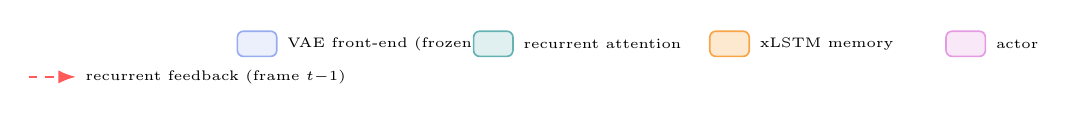
\begin{tikzpicture}[baseline]
    \foreach \s/\t [count=\i] in {vae/VAE front-end (frozen),attn/recurrent attention,mem/xLSTM memory,head/actor\,/\,critic} {
      \node[\s,minimum width=5mm,minimum height=3.2mm] (L\i) at (\i*3.0,0) {};
      \node[anchor=west,font=\tiny] at (L\i.east) {\t};
    }
    \draw[fb] (0.1,-0.42)--(0.7,-0.42); \node[anchor=west,font=\tiny] at (0.7,-0.42){recurrent feedback (frame $t{-}1$)};
  \end{tikzpicture}}
